% Provenance (never printed): enseignement scientifique premiere (2019),
% "La Terre, un astre singulier" (the place of the Earth) and the old seconde
% SVT "La planete Terre, une planete habitable" (conditions for liquid water,
% the habitable zone); see sources/book2/PROVENANCE.md. Every temperature,
% phase boundary and habitable-zone limit is computed in
% figdata/grade-10/planet_temperatures.py.
\chapter{A Habitable Planet}\label{ch:g10:habitable-planet}

Three rocky planets circle the Sun side by side. On the surface of Venus the
air is so dense that it presses ninety-two times harder than on the Earth,
and so hot --- more than \qty{460}{\degreeCelsius} --- that lead would melt.
On Mars the thin air presses less than a hundredth as hard as ours, and the
average temperature is far below freezing. Between them, the Earth has
oceans, rain and life. The three planets formed from the same disc of gas and
dust around the young Sun, out of much the same rock. Why such different
fates? This chapter looks at what sets the temperature of a planet, what lets
it keep an atmosphere, under what conditions water can be liquid, and where,
around the Sun and around other stars, such conditions can be found.
% ledger: nasa:venus-atm, nasa:mars-atm, planet:Venus.Tmean

\begin{omfigure}
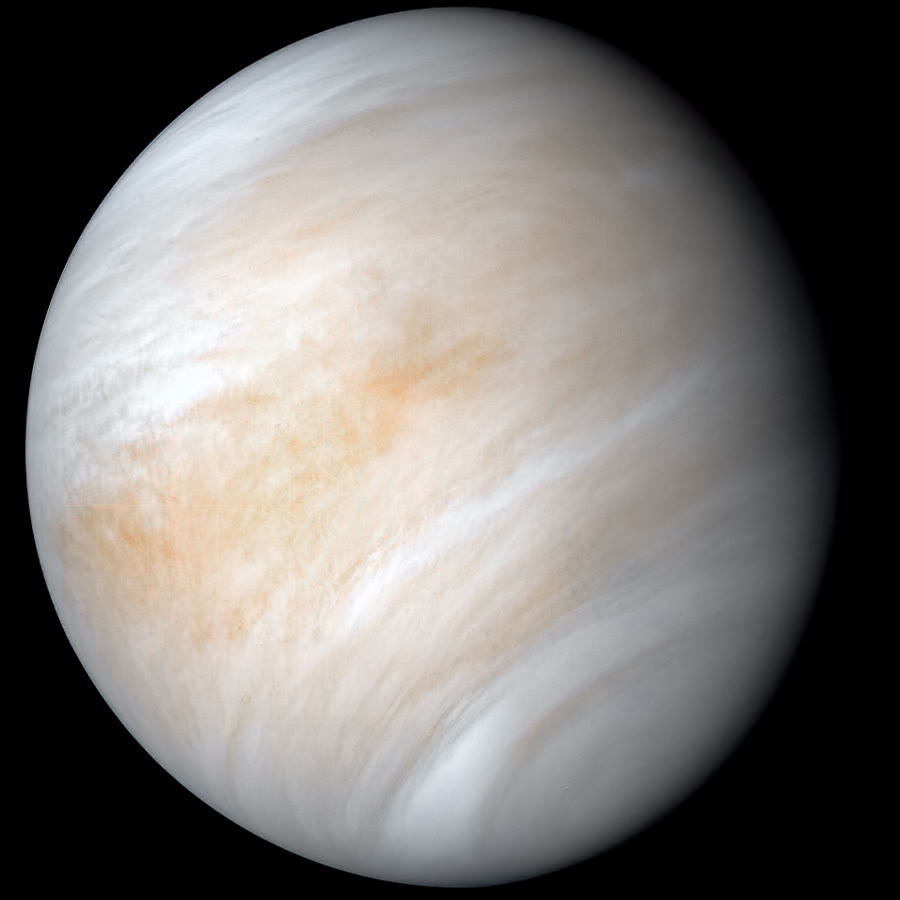
\includegraphics[width=0.38\linewidth]{images/book2/g10-nasa-venus-mariner10.jpg}

{\small Venus seen by the probe Mariner~10 in 1974, in colours close to what
the eye would see: a planet entirely wrapped in cloud. Image: NASA/JPL-Caltech
(public domain).}
\end{omfigure}

\begin{recall}
The Sun is a star; around it the four rocky planets Mercury, Venus, the Earth
and Mars, then the four giant planets, travel on nearly circular orbits
(the physics books and Book 1). Every body radiates energy as light, more and
more of it as its temperature rises, mostly as infrared light at the
temperatures of planets (the physics books). Greenhouse gases --- water
vapour, carbon dioxide, methane --- absorb part of the infrared emitted by a
surface and keep it warmer (the chemistry books). Water exists as ice,
liquid water and water vapour; pressure is a force per unit area, measured in
pascals (the physics books).
\end{recall}

\section{The temperature set by the star}

The Sun sends its light equally in all directions. At a distance $d$, its
power $L$ (its \emph{luminosity}) is spread over a sphere of area $4\pi d^2$.

\begin{proposition}[The inverse-square law of sunlight]\label{prop:g10:habitable-planet:inverse-square}
The power received per square metre facing the Sun, the \emph{solar
irradiance}, at a distance $d$ from the Sun is
\[
  S = \frac{L}{4\pi d^2}.
\]
At the Earth's distance, \qty{1}{au}, $S_0 = \qty{1361}{W/m^2}$; at a
distance $d$ measured in astronomical units, $S = S_0/d^2$.
\end{proposition}

\begin{proof}
No light is lost in empty space, so the whole power $L$ crosses every sphere
centred on the Sun; on a sphere of radius $d$ it is shared among $4\pi d^2$
square metres. Doubling $d$ multiplies the area by four and divides $S$ by
four.
\end{proof}
% ledger: earth:TSI, sun:L, const:au

\begin{omfigure}
\begin{tikzpicture}[font=\small, >={Stealth[length=2mm]}]
  \shade[ball color=yellow!70!orange] (0,0) circle (0.35);
  \node[below=4pt] at (0,-0.35) {Sun};
  \draw[omThm!70, thick] (0,0) -- (3,0.6) (0,0) -- (3,-0.6);
  \draw[omThm!70, thick, dashed] (3,0.6) -- (6,1.2) (3,-0.6) -- (6,-1.2);
  \draw[fill=omDef!25, draw=omDef!80!black] (3,-0.6) rectangle (3.18,0.6);
  \draw[fill=omDef!12, draw=omDef!80!black] (6,-1.2) rectangle (6.18,1.2);
  \draw[omDef!80!black] (6,0) -- (6.18,0) (6.09,-1.2) -- (6.09,1.2);
  \node[anchor=north] at (3.1,-0.7) {$d$};
  \node[anchor=north] at (6.1,-1.3) {$2d$};
  \node[anchor=south east, align=right, font=\footnotesize] at (2.9,0.75) {1 square:\\all the light};
  \node[anchor=west, align=left, font=\footnotesize] at (6.35,0.6) {4 squares:\\a quarter each};
  \draw[->, black!60] (0.5,-1.95) -- (6.1,-1.95);
  \node[anchor=north, font=\footnotesize] at (3.3,-2.0) {distance from the Sun};
\end{tikzpicture}

{\small The light that crosses one square at distance $d$ is spread over four
squares of the same size at distance $2d$: the irradiance falls as the
inverse square of the distance.}
\end{omfigure}

A planet absorbs the part of this light that it does not reflect, and it
radiates energy to space as infrared light. If it absorbs more than it
radiates, it warms up; warmer, it radiates more; it settles at the
temperature where the two balance.

\begin{definition}[Equilibrium temperature]\label{def:g10:habitable-planet:equilibrium-temperature}
The \emph{equilibrium temperature}\index{equilibrium temperature} of a
planet is the temperature at which a body radiating like a perfect emitter
would send to space exactly the power the planet absorbs from its star. The
fraction of the incoming light that the planet reflects as a whole is its
\emph{Bond albedo} $A$.
\end{definition}

\begin{proposition}[Computing the equilibrium temperature]\label{prop:g10:habitable-planet:teq}
For a planet that spreads the heat it absorbs over its whole surface,
\[
  T_{\mathrm{eq}} = \left(\frac{S\,(1-A)}{4\sigma}\right)^{1/4},
  \qquad \sigma = \qty{5.67e-8}{W.m^{-2}.K^{-4}}.
\]
At the Earth's distance and with no reflection at all, this gives
\qty{278.3}{K}; at a distance $d$ in astronomical units and with albedo $A$,
$T_{\mathrm{eq}} = \qty{278.3}{K} \times (1-A)^{1/4}/\sqrt{d}$.
\end{proposition}

\begin{proof}[Partial proof]
The planet intercepts sunlight on a disc of area $\pi R^2$ and absorbs the
power $(1-A)\,S\,\pi R^2$. It radiates from its whole surface, $4\pi R^2$.
A perfect emitter at temperature $T$ radiates $\sigma T^4$ per square
metre (a law proved in the physics books, admitted here). Equating
$4\pi R^2 \sigma T^4 = (1-A)\,S\,\pi R^2$ gives the formula; the radius
cancels. With $S = S_0/d^2$, the fourth root of $1/d^2$ is $1/\sqrt d$.
\end{proof}
% ledger: const:sigma, earth:TSI

\begin{example}[The Earth]\label{ex:g10:habitable-planet:earth}
% ledger: earth:TSI, earth:albedo, earth:Tbb, earth:Tsurf
With $S_0 = \qty{1361}{W/m^2}$ and $A = 0.294$,
$T_{\mathrm{eq}} = 278.3 \times 0.706^{1/4} \approx \qty{255}{K}$, that is
\qty{-18}{\degreeCelsius}. (NASA's fact sheet lists \qty{254}{K}.) The
average temperature of the Earth's surface is \qty{288}{K},
\qty{15}{\degreeCelsius}: the greenhouse effect of the atmosphere warms it by
about \qty{33}{K}. Without it the oceans would freeze.
\end{example}

\begin{omfigure}
\begin{tikzpicture}
\begin{axis}[ybar, width=0.86\linewidth, height=5.8cm, ymin=0, ymax=950,
  bar width=10pt, enlarge x limits=0.15, symbolic x coords={Mercury,Venus,Earth,Moon,Mars},
  xtick=data, ylabel={temperature (K)}, ymajorgrids, grid style={gray!22},
  legend style={at={(0.97,0.95)}, anchor=north east, font=\footnotesize, draw=black!30},
  nodes near coords, nodes near coords style={font=\scriptsize, rotate=90, anchor=west, /pgf/number format/fixed, /pgf/number format/precision=0},
  tick label style={font=\small}, label style={font=\small}]
\addplot[fill=omDef!45, draw=omDef!80!black] table[x=name, y=Teq_K] {figdata/out/grade-10-planet_temperatures-planets.dat};
\addlegendentry{equilibrium temperature}
\addplot[fill=omThm!55, draw=omThm!80!black] table[x=name, y=Tmean_K] {figdata/out/grade-10-planet_temperatures-planets.dat};
\addlegendentry{measured mean surface temperature}
\end{axis}
\end{tikzpicture}

{\small \omterm{def:g10:habitable-planet:equilibrium-temperature}{Equilibrium temperatures} computed from each body's distance and Bond
albedo, beside the measured mean temperatures of their surfaces. Data: NASA
planetary fact sheets.}
\end{omfigure}

\begin{remark}[Reading the chart]\label{rem:g10:habitable-planet:reading}
% ledger: nasa:bond-albedos, planet:Mercury.Tmean, planet:Venus.Tmean, planet:Moon.Tmean, planet:Mars.Tmean, planet:Moon.day, nasa:moon-temps
For Mercury and Mars, which have almost no atmosphere or a very thin one,
the measured mean is close to the \omterm{def:g10:habitable-planet:equilibrium-temperature}{equilibrium temperature}. The Moon's mean
lies below it: its days and nights each last about two weeks, and its
surface swings from about \qty{95}{K} to \qty{390}{K}, which the simple
formula, made for a planet that spreads its heat evenly, does not capture.
Venus is the striking case: with a Bond albedo of 0.77 --- its clouds reflect
most of the sunlight --- its \omterm{def:g10:habitable-planet:equilibrium-temperature}{equilibrium temperature} is lower than the
Earth's, yet its surface is more than \qty{500}{K} hotter than that: the
greenhouse effect of its thick carbon-dioxide atmosphere.
\end{remark}

\section{Holding an atmosphere}

A gas is made of molecules in constant motion, faster the hotter the gas.
A molecule at the top of an atmosphere that moves upwards faster than the
planet's escape speed --- the speed needed to leave its gravity for good
(the physics books) --- is lost to space. Over billions of years, a small
planet with a weak gravity loses its air; a large one keeps it.

\begin{center}
\small
% ledger: planet:Mercury.vesc, planet:Venus.vesc, planet:Earth.vesc, planet:Moon.vesc, planet:Mars.vesc, planet:Mercury.psurf, planet:Venus.psurf, planet:Earth.psurf, planet:Moon.psurf, nasa:mars-atm
\begin{tabular}{lccc}
\hline
body & escape speed (\unit{km/s}) & surface pressure (bar) & atmosphere \\
\hline
Moon & 2.4 & 0 & none \\
Mercury & 4.3 & 0 & none \\
Mars & 5.0 & 0.006 & thin, carbon dioxide \\
Venus & 10.4 & 92 & thick, carbon dioxide \\
Earth & 11.2 & 1 & nitrogen and oxygen \\
\hline
\end{tabular}
\end{center}

\begin{remark}[Size is not the whole story]\label{rem:g10:habitable-planet:size}
The Moon and Mercury, small and (for Mercury) close to the hot Sun, have
lost almost all their gases. Mars, with half the Earth's escape speed, kept a
thin atmosphere. Venus and the Earth have nearly the same size and escape
speed, yet very different atmospheres: their histories --- the fate of their
water and of their carbon dioxide --- diverged, as \cref{ch:g12:early-earth}
will show for the Earth.
\end{remark}

\section{Liquid water}

\begin{omfigure}
\begin{tikzpicture}
\begin{axis}[omrecord, width=0.88\linewidth, height=7.2cm, xmin=150, xmax=800,
  ymode=log, ymin=1e-6, ymax=2000, xlabel={temperature (K)}, ylabel={pressure (bar)},
  xtick={200,300,...,800}, ytick={1e-6,1e-4,1e-2,1,100},
  log basis y=10]
\addplot[omDef!85!black, line width=1.1pt] table[x=T_K, y=p_bar] {figdata/out/grade-10-planet_temperatures-vap.dat};
\addplot[omDef!85!black, line width=1.1pt] table[x=T_K, y=p_bar] {figdata/out/grade-10-planet_temperatures-subl.dat};
\addplot[omDef!85!black, line width=1.1pt] table[x=T_K, y=p_bar] {figdata/out/grade-10-planet_temperatures-melt.dat};
\addplot[only marks, mark=*, mark size=2pt, black] coordinates {(273.16,0.00611657) (647.096,220.64)};
\addplot[only marks, mark=square*, mark size=2.4pt, omThm!85!black] table[x=T_K, y=p_bar] {figdata/out/grade-10-planet_temperatures-points.dat};
\node[font=\small] at (axis cs:205,30) {ice};
\node[font=\small] at (axis cs:420,30) {liquid};
\node[font=\small] at (axis cs:600,1e-3) {water vapour};
\node[font=\footnotesize, anchor=north west] at (axis cs:276,0.0055) {triple point};
\node[font=\footnotesize, anchor=south east] at (axis cs:640,300) {critical point};
\node[font=\footnotesize, anchor=south, omThm!85!black] at (axis cs:737,110) {Venus};
\node[font=\footnotesize, anchor=west, omThm!85!black] at (axis cs:296,1.0) {Earth};
\node[font=\footnotesize, anchor=north, omThm!85!black] at (axis cs:210,0.0045) {Mars};
\end{axis}
\end{tikzpicture}

{\small The phase diagram of water, with the mean surface conditions of
Venus, the Earth and Mars (squares). The pressure axis is logarithmic: each
tick is a hundred times the one below. Curves computed from the equations
of the International Association for the Properties of Water and Steam;
planetary values from NASA.}
\end{omfigure}

\begin{proposition}[When water can be liquid]\label{prop:g10:habitable-planet:liquid}
% ledger: iapws:triple-critical, iapws:vapour-pressure, iapws:melt-subl
Liquid water exists only at pressures above that of the \emph{triple point},
\qty{611.657}{Pa} (\qty{0.006}{bar}), where ice, liquid and vapour coexist
at \qty{273.16}{K}, and at temperatures below the \emph{critical point},
\qty{647.096}{K} (\qty{220.64}{bar}), beyond which liquid and vapour can no
longer be told apart. At a given pressure above the triple point, water is
liquid between its melting point, close to \qty{273}{K}, and its boiling
point, which falls as the pressure falls.
\end{proposition}

\begin{example}[Three planets on one diagram]\label{ex:g10:habitable-planet:three}
% ledger: nasa:venus-atm, nasa:mars-atm, earth:psurf, earth:Tsurf (boiling point at 636 Pa computed)
The Earth's surface, at \qty{288}{K} and \qty{1}{bar}, lies inside the
liquid field: water there can be liquid, ice or vapour as the weather goes.
Venus, at \qty{737}{K}, lies far beyond the critical temperature: no liquid
water is possible at all. Mars, at \qty{6.36}{mbar}, lies just above the
triple point: water there boils at about \qty{0.5}{\degreeCelsius}, so liquid
water could survive only in a window of about half a degree, and the mean
temperature, \qty{210}{K}, is in the ice field.
\end{example}

\begin{omfigure}
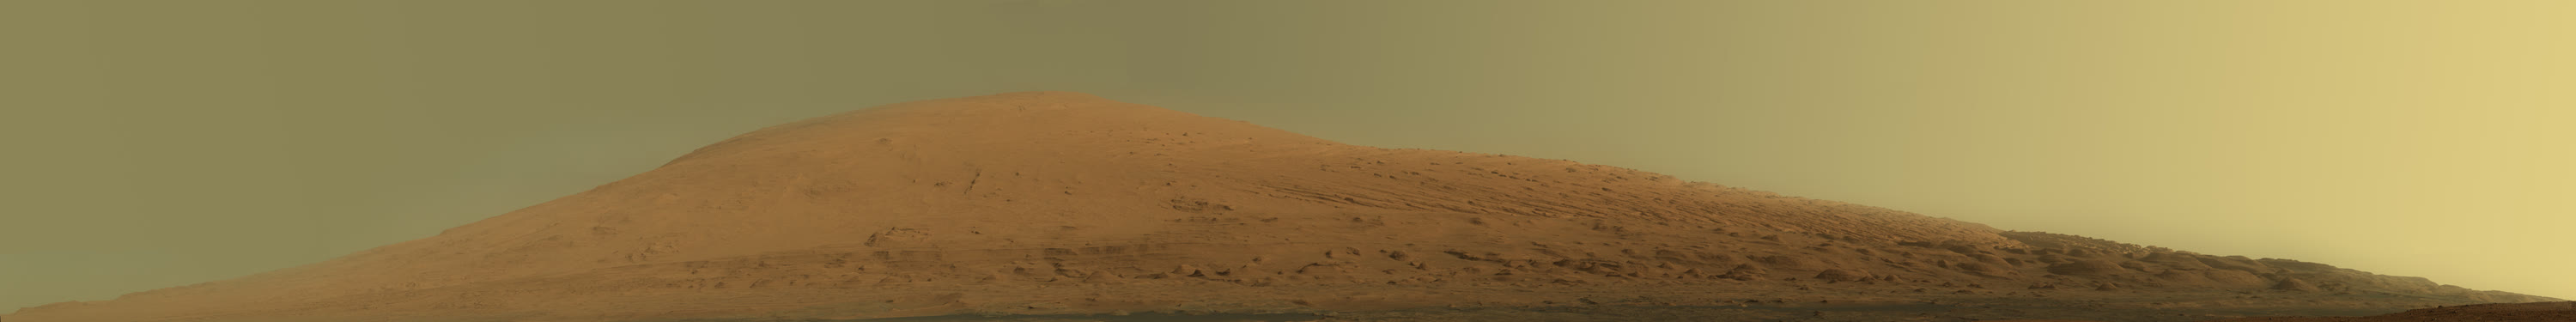
\includegraphics[width=0.96\linewidth]{images/book2/g10-nasa-mars-mount-sharp.jpg}

{\small Mount Sharp, inside Gale Crater on Mars, photographed by the rover
Curiosity in 2012, in the colours recorded by its camera. Its lower layers
were laid down in water, billions of years ago. Image: NASA/JPL-Caltech/MSSS
(public domain).}
\end{omfigure}

\section{The habitable zone}

\begin{definition}[Habitable zone]\label{def:g10:habitable-planet:habitable-zone}
The \emph{habitable zone}\index{habitable zone} of a star is the range of
distances from the star at which a rocky planet with enough water and an
atmosphere like the Earth's could keep liquid water on its surface. Its
inner edge is where the planet would lose its water to the heat; its outer
edge, where even a strong greenhouse effect could no longer keep it from
freezing.
\end{definition}

\begin{proposition}[The Sun's habitable zone]\label{prop:g10:habitable-planet:hz-sun}
% ledger: kopparapu:hz-sun, planet:Mercury.dist, planet:Venus.dist, planet:Mars.dist
Detailed models of planetary atmospheres place the \omterm{def:g10:habitable-planet:habitable-zone}{habitable zone} of the Sun
between \qty{0.99}{au} and \qty{1.70}{au}. The Earth (\qty{1}{au}) lies just
inside its inner edge; Mars (\qty{1.52}{au}) lies inside it; Venus
(\qty{0.72}{au}) lies well inside the inner edge.
\end{proposition}

\begin{proposition}[Habitable zones of other stars]\label{prop:g10:habitable-planet:hz-scaling}
Around a star of luminosity $L$, a planet receives the same irradiance as at
a distance $d_\odot$ from the Sun when it lies at
\[
  d = d_\odot \sqrt{L/L_\odot}.
\]
The edges of the \omterm{def:g10:habitable-planet:habitable-zone}{habitable zone} move in proportion, to a first
approximation (the colour of the star's light also matters a little).
\end{proposition}

\begin{proof}
Equal irradiance means $L/(4\pi d^2) = L_\odot/(4\pi d_\odot^2)$, so
$d^2 = d_\odot^2\,L/L_\odot$.
\end{proof}

\begin{omfigure}
\begin{tikzpicture}[font=\small]
  % top: the Sun, 0-2 au over 12 cm (6 cm per au)
  \fill[omProp!30] (0.99*6,0) rectangle (1.70*6,0.5);
  \draw[black!70] (0,0.25) -- (12.3,0.25);
  \foreach \x in {0,0.5,...,2} \draw (\x*6,0.15) -- (\x*6,0.35) node[pos=0, below=1pt, font=\footnotesize] {\x};
  \shade[ball color=yellow!70!orange] (0,0.25) circle (0.22);
  \foreach \n/\d in {Mercury/0.387, Venus/0.723, Earth/1.0, Mars/1.524} {
    \fill[omThm!85!black] (\d*6,0.25) circle (2.2pt);
    \node[anchor=south, font=\footnotesize] at (\d*6,0.55) {\n};
  }
  \node[anchor=west, font=\footnotesize] at (12.4,0.25) {au};
  \node[anchor=north, font=\footnotesize] at (8.07,-0.25) {habitable zone, 0.99--1.70 au};
  \node[anchor=east, font=\footnotesize] at (-0.3,0.25) {Sun};
  % bottom: Proxima Centauri, 0-0.1 au over 12 cm (120 cm per au)
  \begin{scope}[yshift=-2.2cm]
  \fill[omProp!30] (0.0385*120,0) rectangle (0.0661*120,0.5);
  \draw[black!70] (0,0.25) -- (12.3,0.25);
  \foreach \x/\l in {0/0, 0.025/0.025, 0.05/0.05, 0.075/0.075, 0.1/0.1} \draw (\x*120,0.15) -- (\x*120,0.35) node[pos=0, below=1pt, font=\footnotesize] {\l};
  \shade[ball color=red!70!orange] (0,0.25) circle (0.14);
  \fill[omThm!85!black] (0.0485*120,0.25) circle (2.2pt);
  \node[anchor=south, font=\footnotesize] at (0.0485*120,0.55) {Proxima b};
  \node[anchor=west, font=\footnotesize] at (12.4,0.25) {au};
  \node[anchor=north, font=\footnotesize] at (6.28,-0.25) {habitable zone, 0.038--0.066 au};
  \node[anchor=east, align=right, font=\footnotesize] at (-0.3,0.25) {Proxima\\Centauri};
  \end{scope}
\end{tikzpicture}

{\small Top: the \omterm{def:g10:habitable-planet:habitable-zone}{habitable zone} of the Sun and the four rocky planets. Bottom:
the \omterm{def:g10:habitable-planet:habitable-zone}{habitable zone} of the faint red star Proxima Centauri, computed by
scaling the Sun's with the square root of the star's luminosity, and its
planet Proxima~b. Note the change of scale: the whole bottom strip is
\qty{0.1}{au} long.}
\end{omfigure}

\section{Planets of other stars}

\begin{definition}[Exoplanet]\label{def:g10:habitable-planet:exoplanet}
An \emph{exoplanet}\index{exoplanet} is a planet that orbits a star other
than the Sun.
\end{definition}

\omterm{def:g10:habitable-planet:exoplanet}{Exoplanets} are far too faint and too close to their stars to be seen
directly, apart from a few giants. Most are found indirectly: either the
planet passes in front of its star once per orbit and dims it very slightly,
or its pull makes the star wobble towards and away from us, which shifts the
colour of the star's light back and forth. The second method gives only a
\emph{minimum} mass for the planet, because the tilt of the orbit is not
known. These methods are studied in the Year~3 volume.

\begin{dated}{2026}
% ledger: nea:count-2026
On 15 October 2026 the NASA \omterm{def:g10:habitable-planet:exoplanet}{Exoplanet} Archive listed 6\,451 confirmed
\omterm{def:g10:habitable-planet:exoplanet}{exoplanets}.
\end{dated}

\begin{example}[Proxima b]\label{ex:g10:habitable-planet:proxima}
% ledger: nea:proxima-b (flux and habitable zone computed in figdata/grade-10/planet_temperatures.py)
The nearest star to the Sun, Proxima Centauri, \qty{1.30}{\parsec} away, is a
small red star whose luminosity is only about $0.0015$ that of the Sun. In
2016 a planet was found orbiting it every 11.2 days, at \qty{0.0485}{au},
with at least 1.06 times the mass of the Earth. At that distance it receives
about 0.64 of the irradiance the Earth receives, and it lies inside its
star's \omterm{def:g10:habitable-planet:habitable-zone}{habitable zone}. Whether it has an atmosphere, or water, is not known.
\end{example}

\begin{remark}[Habitable is not inhabited]\label{rem:g10:habitable-planet:inhabited}
The \omterm{def:g10:habitable-planet:habitable-zone}{habitable zone} is a statement about distance and light only. A planet
inside it may have no water, no atmosphere, or the wrong one --- Mars lies
inside the Sun's zone and has no liquid water at its surface today. The Earth
is habitable because several conditions hold at once: the right distance, a
mass large enough to keep an atmosphere, abundant water, and a greenhouse
effect neither too weak nor too strong.
\end{remark}

\section{Exercises}

\begin{exercise}[$\star$]\label{exo:g10:habitable-planet:1}
Define the \omterm{def:g10:habitable-planet:equilibrium-temperature}{equilibrium temperature} of a planet. Why is the Earth's mean
surface temperature higher than its \omterm{def:g10:habitable-planet:equilibrium-temperature}{equilibrium temperature}?
\end{exercise}

\begin{exercise}[$\star$]\label{exo:g10:habitable-planet:2}
Using the bar chart of equilibrium and measured temperatures, name the body
whose surface is warmed most by its atmosphere, and estimate by how many
kelvins.
\end{exercise}

\begin{exercise}[$\star$]\label{exo:g10:habitable-planet:3}
Mars orbits at \qty{1.52}{au} from the Sun. Using the inverse-square law with
$S_0 = \qty{1361}{W/m^2}$, compute the solar irradiance at Mars.
\end{exercise}

\begin{exercise}[$\star$]\label{exo:g10:habitable-planet:4}
Using the phase diagram of water, give the state of water at \qty{1}{bar}
and \qty{330}{K}; at \qty{0.001}{bar} and \qty{250}{K}; at \qty{100}{bar} and
\qty{700}{K}.
\end{exercise}

\begin{exercise}[$\star$]\label{exo:g10:habitable-planet:5}
What is an \omterm{def:g10:habitable-planet:exoplanet}{exoplanet}? Describe in one sentence each the two main ways in
which \omterm{def:g10:habitable-planet:exoplanet}{exoplanets} are detected.
\end{exercise}

\begin{exercise}[$\star\star$]\label{exo:g10:habitable-planet:6}
Compute the Earth's \omterm{def:g10:habitable-planet:equilibrium-temperature}{equilibrium temperature} with $S_0 = \qty{1361}{W/m^2}$
and $A = 0.294$, then with $A = 0$. Convert both to degrees Celsius.
\end{exercise}

\begin{exercise}[$\star\star$]\label{exo:g10:habitable-planet:7}
A star is four times as luminous as the Sun. Between which distances does
its \omterm{def:g10:habitable-planet:habitable-zone}{habitable zone} lie? Would the Earth, placed at \qty{1}{au} from it, be
inside?
\end{exercise}

\begin{exercise}[$\star\star$]\label{exo:g10:habitable-planet:8}
Venus orbits at \qty{0.723}{au}. Compute the irradiance it receives, then its
\omterm{def:g10:habitable-planet:equilibrium-temperature}{equilibrium temperature} with its Bond albedo of 0.77. Compare with its
surface temperature of \qty{737}{K} and explain the difference.
\end{exercise}

\begin{exercise}[$\star\star$]\label{exo:g10:habitable-planet:9}
On Mars the mean surface pressure is \qty{6.36}{mbar}, just above the triple
point of water, and water boils there at about \qty{0.5}{\degreeCelsius}.
Explain why liquid water cannot last on the surface of Mars today, even on a
summer afternoon when the ground reaches \qty{10}{\degreeCelsius}.
\end{exercise}

\begin{exercise}[$\star\star$]\label{exo:g10:habitable-planet:10}
The escape speed is \qty{2.4}{km/s} on the Moon and \qty{11.2}{km/s} on the
Earth. Compute their ratio. Explain why the Earth has kept an atmosphere and
the Moon has not.
\end{exercise}

\begin{exercise}[$\star\star$]\label{exo:g10:habitable-planet:11}
Suppose the Earth were covered with ice and its Bond albedo rose to 0.50.
Compute its new \omterm{def:g10:habitable-planet:equilibrium-temperature}{equilibrium temperature}. Explain why such a state, once
reached, would tend to last.
\end{exercise}

\begin{exercise}[$\star\star\star$]\label{exo:g10:habitable-planet:12}
Show that $T_{\mathrm{eq}} = \qty{278.3}{K} \times (1-A)^{1/4}/\sqrt{d}$, with
$d$ in astronomical units, follows from the formula of the chapter. By what
factor does the \omterm{def:g10:habitable-planet:equilibrium-temperature}{equilibrium temperature} change when the distance is
multiplied by four?
\end{exercise}

\begin{exercise}[$\star\star\star$]\label{exo:g10:habitable-planet:13}
At what distance from the Sun would a planet of albedo 0.294 have an
\omterm{def:g10:habitable-planet:equilibrium-temperature}{equilibrium temperature} of \qty{273}{K}? Compare with the inner edge of the
\omterm{def:g10:habitable-planet:habitable-zone}{habitable zone}, and explain why the two are different.
\end{exercise}

\begin{exercise}[$\star\star\star$]\label{exo:g10:habitable-planet:14}
On a planet whose surface pressure is \qty{1000}{Pa}, water boils at about
\qty{7}{\degreeCelsius}. Between which temperatures can water be liquid
there? What would happen to a lake on that planet on a day at
\qty{15}{\degreeCelsius}?
\end{exercise}

\begin{exercise}[$\star\star\star$]\label{exo:g10:habitable-planet:15}
A planet orbits at \qty{1.2}{au} from a star half as luminous as the Sun.
Compute the edges of the star's \omterm{def:g10:habitable-planet:habitable-zone}{habitable zone} and say whether the planet is
inside. How sure can one be of the answer?
\end{exercise}

\section{Problem: Could Proxima b Hold an Ocean?}

\begin{problem}[{Weekend problem --- from the light of a faint red star to
the temperature of its nearest planet}]
\label{pb:g10:habitable-planet:1}
% ledger: nea:proxima-b, kopparapu:hz-sun, earth:TSI, earth:albedo, planet:Earth.vesc, nasa:bond-albedos (all results computed in figdata/grade-10/planet_temperatures.py or from the rounded data below)
A student reads the data sheet of the planet Proxima~b. Its star has a
luminosity $L = 0.00151\,L_\odot$; the planet orbits at $d = \qty{0.0485}{au}$
in 11.18 days and has at least 1.055 times the mass of the Earth. Use
$S_0 = \qty{1361}{W/m^2}$, $\sigma = \qty{5.67e-8}{W.m^{-2}.K^{-4}}$, the
Sun's \omterm{def:g10:habitable-planet:habitable-zone}{habitable zone} \qtyrange{0.99}{1.70}{au}, and the Earth's escape speed
\qty{11.2}{km/s}.

\medskip
\noindent\textbf{Part I --- The light of the star.}
\begin{enumerate}
  \item Compute the irradiance at the planet as a fraction of the Earth's,
        $L/d^2$ (with $L$ in solar luminosities and $d$ in au).
  \item Express it in \unit{W/m^2}.
  \item Compare it with the irradiance at Venus (\qty{2601}{W/m^2}) and at
        Mars (\qty{586}{W/m^2}).
  \item How many of the planet's years fit into one Earth year?
\end{enumerate}

\medskip
\noindent\textbf{Part II --- Temperatures without an atmosphere.}
\begin{enumerate}[resume]
  \item Compute the \omterm{def:g10:habitable-planet:equilibrium-temperature}{equilibrium temperature} of a perfectly dark planet
        ($A = 0$) at that irradiance.
  \item Compute it for a planet as bright as Venus ($A = 0.77$).
  \item Which of these two temperatures is above the freezing point of
        water? What do the two results show about the role of clouds and
        ice?
\end{enumerate}

\medskip
\noindent\textbf{Part III --- The habitable zone.}
\begin{enumerate}[resume]
  \item Compute $\sqrt{L/L_\odot}$.
  \item Compute the inner edge of the star's \omterm{def:g10:habitable-planet:habitable-zone}{habitable zone}.
  \item Compute its outer edge.
  \item Is Proxima~b inside the \omterm{def:g10:habitable-planet:habitable-zone}{habitable zone}?
  \item At what distance from the Sun would a planet receive the same
        irradiance as Proxima~b? Where would that be in the Sun's \omterm{def:g10:habitable-planet:habitable-zone}{habitable
        zone}?
\end{enumerate}

\medskip
\noindent\textbf{Part IV --- An atmosphere and water?}
\begin{enumerate}[resume]
  \item If the planet had the Earth's mean density, its radius would be
        $1.055^{1/3}$ times the Earth's. Compute this factor.
  \item The escape speed is proportional to $\sqrt{M/R}$. Estimate the
        planet's escape speed. Could it keep an atmosphere?
  \item Why is the mass known only as a minimum?
  \item On the phase diagram, what is the lowest surface pressure that would
        allow liquid water at all?
  \item Compute the \omterm{def:g10:habitable-planet:equilibrium-temperature}{equilibrium temperature} of Proxima~b with the Earth's
        albedo, 0.294.
  \item By how many kelvins would its greenhouse effect then have to warm
        it to bring its surface to the Earth's mean temperature,
        \qty{288}{K}?
\end{enumerate}
\end{problem}
